\chapter{Irréversibilité et exergie}
Les irréversibilités obligent à utiliser pleins de rendements fonctions d'une 
transformation idéale de référence. Ici, on va définir une transfo réversible de 
référence indépendante du dispositif et ce pour plus de facilité.

	\section{Travail réversible et irréversibilité}
	Le travail (ir)réversible repose sur l'existence d'une source de chaleur 
	gratuite à température $T_0$.
	
		\subsection{Systèmes fermés}
			\begin{wrapfigure}[13]{l}{6.5cm}
%	\vspace{-5mm}
	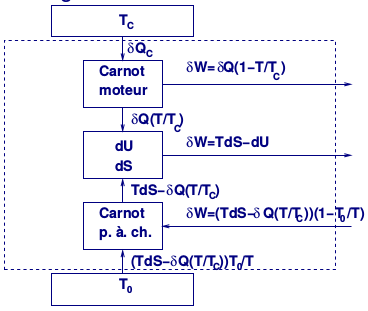
\includegraphics[scale=0.45]{ch8/image1.png}
	\captionof{figure}{ }
	\end{wrapfigure}
		Soit un système fermé recevant $_1Q_2$ d'une source $T_C$ et fournissant 
		un travail $_1W_2^*$. Considérons les deux premiers principes\footnote{Pour 
		l'entropie totale, il s'agit du système + source.}
		\begin{equation}
		\begin{array}{ll}
		_1Q_2 &= U_2-U_1 + _1W_2^*\\
		\Delta S_{tot} &= S_2-S_1 - \dfrac{_1Q_2}{T_C}>0
		\end{array}
		\end{equation}
		Si on ajoute au cycle de Carnot un moteur entre la source chaude et le 
		système et un frigo entre le système et la source froide gratuite, on a 
		créé un système semblable à celui décrit ci-dessus. Il faut toujours veiller 
		à avoir $\delta Q_{sys} = TdS$, soit une transformation réversible. Pour se 
		faire, quand le moteur "consomme" $\delta Q(T/T_C)$, la pompe à chaleur doit 
		compléter cette absorption.\\
		Sommons les travaux des trois systèmes 
		\begin{equation}
		\delta W_{rev}^* = TdS - dU + \delta Q\left(1-\dfrac{T}{T_C}\right)-\left(
		T_dS - \delta Q \dfrac{T}{T_C}\right)\left(1-\dfrac{T_0}{T}\right) = T_0dS - dU + 
		\delta Q\left(1-\dfrac{T_0}{T_C}\right)
		\end{equation}
		En intégrant, pour une transformation finie :
		\begin{equation}
		W_{rev}^* =T_0(S_2-S_1) - (U_2-U_1) + _1Q_2\left(1-\dfrac{T_0}{T_C}\right)
		\end{equation}
		La différence entre le travail réalisé et le réversible est l'irréversibilité :
		\begin{equation}
		_1I_2 = W_{rev}^* - _1W_2^*
		\end{equation}
		En injectant ce résultat dans l'expression du travail réversible et réel :
		\begin{equation}
		_1I_2 = T_0(S_2-S_1)-_1Q_2\dfrac{T_0}{T_C} = T_0\Delta S_{tot}
		\end{equation}
		On peut le ré-écrire 
		\begin{equation}
		(U_2-U_1) - T_0(S_2-S_1) = _1W_2 + _1Q_2\left(1-\dfrac{T_0}{T_C}\right)-_1I_2
		\end{equation}
		qui ressemble au premier principe, mais avec les irréversibilités. L'énergie 
		utilisable, membre de gauche, est la somme du travail reçu diminué par les 
		pertes irréversibles.
		
		\subsection{Systèmes ouverts en régime permanent}
		L'analyse est identique mais on considère cette fois les systèmes ouvert 
		dans le cas d'une seule section d'entrée/sortie. On trouve alors
		\begin{equation}
		w_{rev}^* = T_0(s_s-s_e) - \left[\left(h_s+\dfrac{c_s^2}{2}+gz_s\right)-
		\left(h_e+\dfrac{c_e^2}{2}+gz_e\right)\right] + q\left(1-\dfrac{T_0}{T_C}\right)
		\label{eq:TravIrr}
		\end{equation}
		L'irréversibilité (cette fois massique) vaut (même raisonnement) 
		\begin{equation}
		i = w_{rev}^* - w^* = T_0(s_s-s_e) - \dfrac{T_0}{T_C}q = T_0\left[\dfrac{1}{
		\dot{m}}\dfrac{dS_{tot}}{dt}\right]
		\end{equation}
		Il est intéressant de réécrire ce résultat comme tel :
		\begin{equation}
		h_s-h_e - T_0(s_s-s_e) + \dfrac{c_s^2-c_e^2}{2}+g(z_s-z_e) = w + q\left(
		1-\dfrac{T_0}{T_C}\right) - i
		\end{equation}
		qui est le \textbf{bilan exergétique} avec $h-T_0s$ l'\textbf{exergie} ou 
		\textbf{enthalpie utilisable}. Ce bilan exprime la conservation de l'exergie, 
		aux pertes d'irréversibilité près. On peut généraliser sans peine en plaçant 
		des $\sum$ un peu partout.\\
		Pour conclure :
		\begin{enumerate}
		\item Puissance mécanique : flux d'exergie pure
		\item Apport exergétique < quantité de chaleur reçue
		\item Apport matière : apport d'exergie valant $j = h-T_0s$
		\item $T$ et $V$ : exergie pure
		\item Irréversibilité : perte d'exergie valant le produit de la production 
		d'entropie totale par le température de la source gratuire.
		\begin{equation}
		I = T_0\Delta S_{tot}
		\end{equation}
		\end{enumerate}
		
		\subsection{Cas général : transformations instationnaires des systèmes ouvert}
		\textit{Vous savez le faire vous-même, je ne le vois pas en cours ce n'est 
		pas intéressant.} Pour les conquérants : slide 219-221.
		
		
	\newpage
	\section{Exergie et rendement exergétique des systèmes ouverts stationnaires}
	Essayons d’interpréter physiquement ces bilans fraîchement obtenus. Soit une 
	quantité de matière dans un état donné. Quel est le travail maximum que cette 
	matière peut fournir dans un système ouvert stationnaire (milieu extérieur : 
	$T_0,p_0$).\\
	Le travail maximum s'obtient en amenant cette quantité de matière en équilibre 
	avec le milieu extérieur. Le travail réversible \autoref{eq:TravIrr} vaut\footnote{
	Il ne manque pas un terme d'énergie cinétique ? Ou considérée nulle dans le milieu extérieur?} :
	\begin{equation}
	w_{rev}^* = \left[\left(h_e-T_0s_e+\dfrac{c_e^2}{2}+gz_e\right) - \left(h_0-T_0s_0
	+gz_0\right)\right] + q\left(1-\dfrac{T_0}{T_C}\right)
	\end{equation}
	Le dernier terme est nul car les seuls échanges de chaleur possibles sont à $T_0$. 
	Le travail max réalisable n'et que la différence d'énergie totale ($T$ et $V$ compris) 
	entre l'état considéré et le milieu extérieur.\\
	On définit parfois l'exergie :
	\begin{equation}
	j \equiv (h-h_0) - T_0(s-s_0)
	\end{equation}
	Si c'est le cas, l'exergie du milieu extérieur est nulle et l'exergie totale 
	correspond au travail maximum réalisé ; elle détermine le travail maximum. Vérifions 
	pour une transformation composée d'une adabatique réversible jusqu'à la température 
	du milieu extérieur suivi d'une isotherme réversible. Si on néglige $T$ et $V$ et 
	en notant $m$, le point intermédiaire $s_m=s_e, T_m=T_0$ :
	\begin{enumerate}
	\item \textit{isentropique} : $w_{rev}^* = h_e-h_m$
 	\item \textit{isotherme} : $h_m-h_0 + T_0(s_0-s_m)$
	\end{enumerate}
	En sommant
	\begin{equation}
	w_{rev}^* = h_e-h_0 - T_0(s_e-s_0) = j_e
	\end{equation}
	L'irréversibilité est liée à la perte de chaleur et à la combustion en elle-même (
	ainsi que l'échange de chaleur à l'extérieur). En effet, si on désire régénérer 
	le charbon à partir de la chaleur ce n'est pas possible. C'est irréversible, on a 
	produit un $\Delta S$. Ceci montre que la combusion est une "perte".\\
	
	Forcément, moins il y a d'irréversibilité, plus grand est le travail effectué. Donc 
	plus de pertes = plus de diminution d'exergie. On définit ainsi un rendement exergétique :
	\begin{equation}
	\eta_{ex} = \dfrac{\text{variation d'exergie utile réelle}}{\text{variation d'exergie 
	utile réversible}}
	\end{equation}
	Pour les différents rendements, référez-vous au formulaire.
		
		
		
		
		
		
		
		
		
		
		
		
		
		
		
		
		
		
		
		
		
		
		
		
		
		
		
		
		
		
		
		
		
		
		
		
		
		
		
		
		
		
		
		
